\documentclass[12pt]{article}
    \usepackage{tikz}
    
    \begin{document}
    
    \begin{center}
    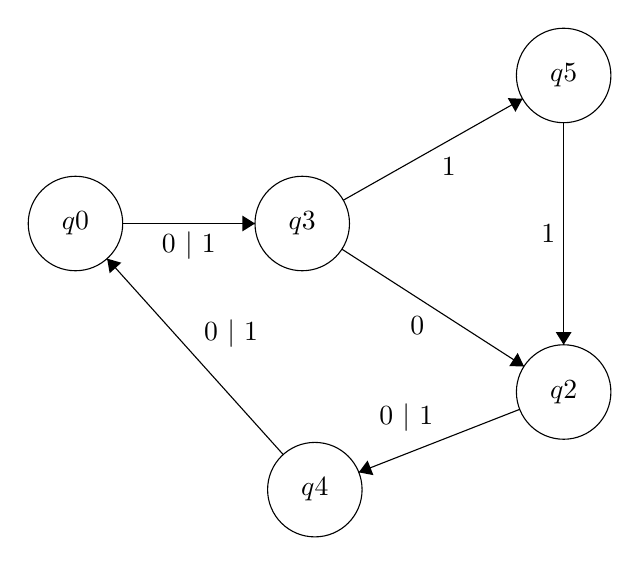
\begin{tikzpicture}[scale=0.2]
    \tikzstyle{every node}+=[inner sep=0pt]
    \draw [black] (11,-26.7) circle (3);
    \draw (11,-26.7) node {$q0$};
    \draw [black] (42,-17.3) circle (3);
    \draw (42,-17.3) node {$q5$};
    \draw [black] (25.4,-26.7) circle (3);
    \draw (25.4,-26.7) node {$q3$};
    \draw [black] (42,-37.4) circle (3);
    \draw (42,-37.4) node {$q2$};
    \draw [black] (26.2,-43.6) circle (3);
    \draw (26.2,-43.6) node {$q4$};
    \draw [black] (14,-26.7) -- (22.4,-26.7);
    \fill [black] (22.4,-26.7) -- (21.6,-26.2) -- (21.6,-27.2);
    \draw (18.2,-27.2) node [below] {$0\mbox{ }|\mbox{ }1$};
    \draw [black] (28.01,-25.22) -- (39.39,-18.78);
    \fill [black] (39.39,-18.78) -- (38.45,-18.74) -- (38.94,-19.61);
    \draw (34.7,-22.5) node [below] {$1$};
    \draw [black] (42,-20.3) -- (42,-34.4);
    \fill [black] (42,-34.4) -- (42.5,-33.6) -- (41.5,-33.6);
    \draw (41.5,-27.35) node [left] {$1$};
    \draw [black] (27.92,-28.33) -- (39.48,-35.77);
    \fill [black] (39.48,-35.77) -- (39.08,-34.92) -- (38.54,-35.76);
    \draw (32.7,-32.55) node [below] {$0$};
    \draw [black] (39.21,-38.5) -- (28.99,-42.5);
    \fill [black] (28.99,-42.5) -- (29.92,-42.68) -- (29.55,-41.75);
    \draw (32.01,-39.96) node [above] {$0\mbox{ }|\mbox{ }1$};
    \draw [black] (24.19,-41.37) -- (13.01,-28.93);
    \fill [black] (13.01,-28.93) -- (13.17,-29.86) -- (13.91,-29.19);
    \draw (19.14,-33.69) node [right] {$0\mbox{ }|\mbox{ }1$};
    \end{tikzpicture}
    \end{center}
    
    \end{document}
    